\fancyhead[LE]{\fontsize{8.5pt}{10pt}\selectfont\textbf{\textsf{24}}\quad \textbf{\textsf{CHƯƠNG 1}}\quad \textsf{Các hàm số và Mô hình}}
\fancyhead[RO]{\fontsize{8.5pt}{10pt}\selectfont\textsf{MỤC 1.2}\quad \textbf{\textsf{24}}}

\noindent
\begin{minipage}[t]{0.265\textwidth}
    \fontsize{8pt}{10.5pt}\selectfont
    \vspace{150pt}
    
    Máy tính hoặc máy tính bỏ túi có chức năng vẽ đồ thị tìm đường hồi quy bằng \textbf{phương pháp bình phương tối thiểu}, tức là cực tiểu hóa tổng các bình phương khoảng cách thẳng đứng giữa các điểm dữ liệu và đường thẳng. Chi tiết được giải thích trong Bài tập 14.7.61.

    \vspace{45pt}
    \begin{center}
        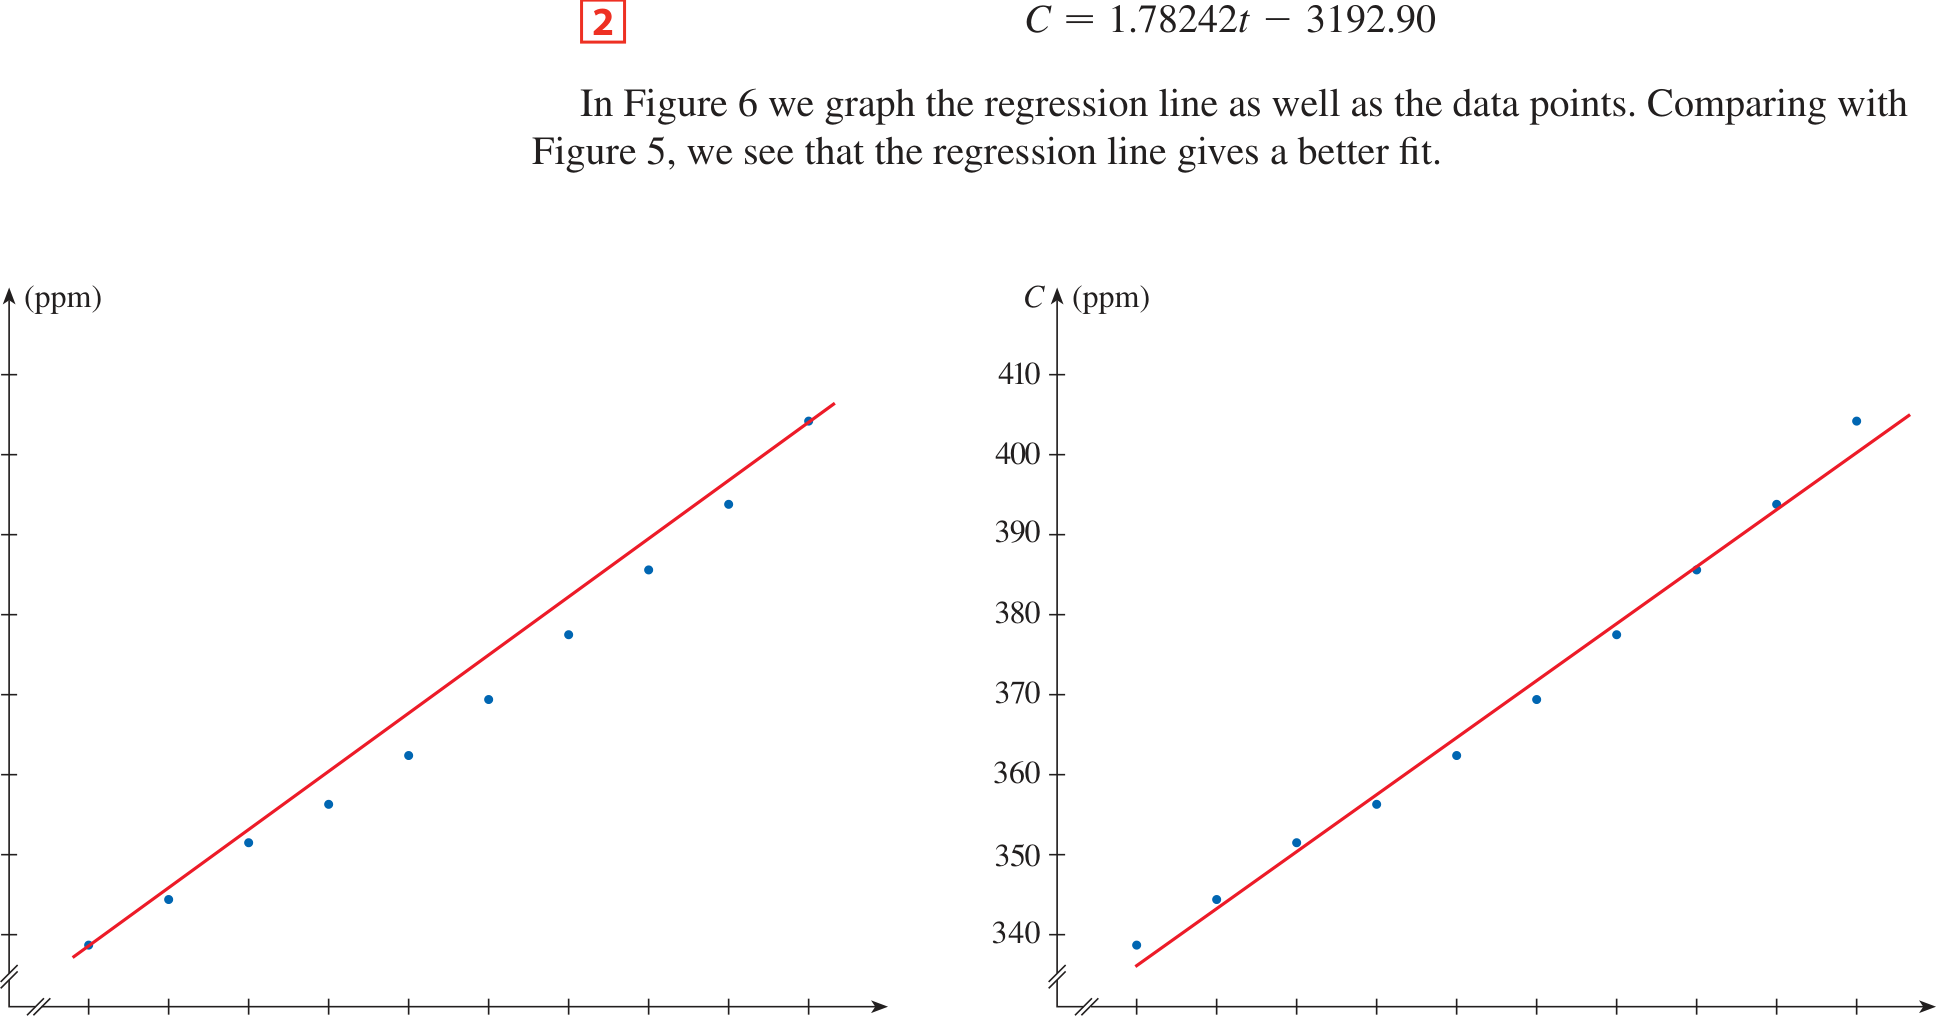
\includegraphics[width=0.92\linewidth]{images/p0059_fig6.png}
        \vspace{2mm}
        
        \raggedright
        \textbf{\textsf{HÌNH 6}}\\[1mm]
        {\fontsize{7.5pt}{9.5pt}\selectfont Đường hồi quy}
    \end{center}
\end{minipage}%
\hfill
\begin{minipage}[t]{0.708\textwidth}
    \fontsize{9.3pt}{13.2pt}\selectfont
    Để ý rằng các điểm dữ liệu dường như nằm sát một đường thẳng, vì vậy việc chọn một mô hình tuyến tính trong trường hợp này là rất tự nhiên. Tuy nhiên, có nhiều đường thẳng khả dĩ có thể xấp xỉ các điểm dữ liệu này, vậy chúng ta nên sử dụng đường thẳng nào? Một khả năng là đường thẳng đi qua điểm dữ liệu đầu tiên và điểm dữ liệu cuối cùng. Hệ số góc của đường thẳng này là
    \[
    \frac{404.2 - 338.7}{2016 - 1980} = \frac{65.5}{36} \approx 1.819
    \]
    Ta viết phương trình của nó dưới dạng
    \[
    C - 338.7 = 1.819(t - 1980)
    \]
    hay
    \begin{equation}
        C = 1.819t - 3262.92
        \tag*{\tikz[baseline=(char.base)]{\node[draw=stewartred, inner sep=1.8pt, line width=0.6pt, rounded corners=0.5pt] (char) {\fontsize{8pt}{9pt}\selectfont\bfseries\color{stewartred} 1};}}
    \end{equation}

    Phương trình 1 cho ta một mô hình tuyến tính khả dĩ cho nồng độ carbon dioxide; mô hình này được vẽ ở Hình 5. Chú ý rằng mô hình của chúng ta cho các giá trị cao hơn phần lớn các mức $\text{CO}_2$ thực tế. Một mô hình tuyến tính tốt hơn có thể nhận được từ một quy trình trong thống kê gọi là \textit{hồi quy tuyến tính}. Nhiều loại máy tính bỏ túi có chức năng vẽ đồ thị và phần mềm máy tính có thể xác định đường hồi quy cho một tập dữ liệu. Một máy tính như vậy cho hệ số góc và giao điểm với trục tung của đường hồi quy đối với dữ liệu từ Bảng 1 là
    \[
    m = 1.78242 \qquad b = -3192.90
    \]
    Do đó, mô hình bình phương tối thiểu của chúng ta cho nồng độ $\text{CO}_2$ là
    \begin{equation}
        C = 1.78242t - 3192.90
        \tag*{\tikz[baseline=(char.base)]{\node[draw=stewartred, inner sep=1.8pt, line width=0.6pt, rounded corners=0.5pt] (char) {\fontsize{8pt}{9pt}\selectfont\bfseries\color{stewartred} 2};}}
    \end{equation}

    Trong Hình 6, chúng ta vẽ đường hồi quy cùng với các điểm dữ liệu. So sánh với Hình 5, ta thấy rằng đường hồi quy khớp tốt hơn.

    \vspace{4mm}
    \begin{center}
        \begin{tikzpicture}[x=0.145cm, y=0.052cm]
            % Trục hoành và trục tung
            \draw[->, >=stealth, semithick] (1976, 335) -- (2019, 335) node[below right] {\fontsize{8pt}{9pt}\selectfont $t$};
            \draw[->, >=stealth, semithick] (1977, 333) -- (1977, 418) node[above right] {\fontsize{8pt}{9pt}\selectfont $C\text{ (ppm)}$};
            
            % Ngắt trục
            \draw[thick] (1977.5, 333) -- (1979, 337);
            \draw[thick] (1978.5, 333) -- (1980, 337);
            \draw[thick] (1975.5, 335.5) -- (1978.5, 337);
            \draw[thick] (1975.5, 337.5) -- (1978.5, 339);

            % Vạch chia trục hoành
            \foreach \x in {1980, 1984, 1988, 1992, 1996, 2000, 2004, 2008, 2012, 2016} {
                \draw (\x, 335) -- (\x, 337);
                \node[below, font=\fontsize{6.5pt}{7.5pt}\selectfont] at (\x, 334) {\x};
            }
            
            % Vạch chia trục tung
            \foreach \y in {340, 350, 360, 370, 380, 390, 400, 410} {
                \draw (1977, \y) -- (1978.5, \y);
                \node[left, font=\fontsize{6.5pt}{7.5pt}\selectfont] at (1976.5, \y) {\y};
            }
            
            % Đường thẳng màu đỏ
            \draw[red, thick] (1978, 335.08) -- (2017.5, 406.9);
            
            % Các điểm dữ liệu
            \foreach \pt in {
                (1980, 338.7),
                (1984, 344.4),
                (1988, 351.5),
                (1992, 356.4),
                (1996, 362.6),
                (2000, 369.4),
                (2004, 377.5),
                (2008, 385.6),
                (2012, 393.8),
                (2016, 404.2)
            } {
                \fill[stewartcyan!80!blue] \pt circle (1.2pt);
            }
        \end{tikzpicture}
        \vspace{2mm}
        
        \raggedright
        \textbf{\textsf{HÌNH 5}}\\[1mm]
        {\fontsize{8.5pt}{10.5pt}\selectfont Mô hình tuyến tính đi qua điểm dữ liệu đầu và cuối}
        \hfill{\color{stewartcyan}$\blacksquare$}
    \end{center}
\end{minipage}